\subsection*{separate rings}

\begin{figure}[H]
\centering
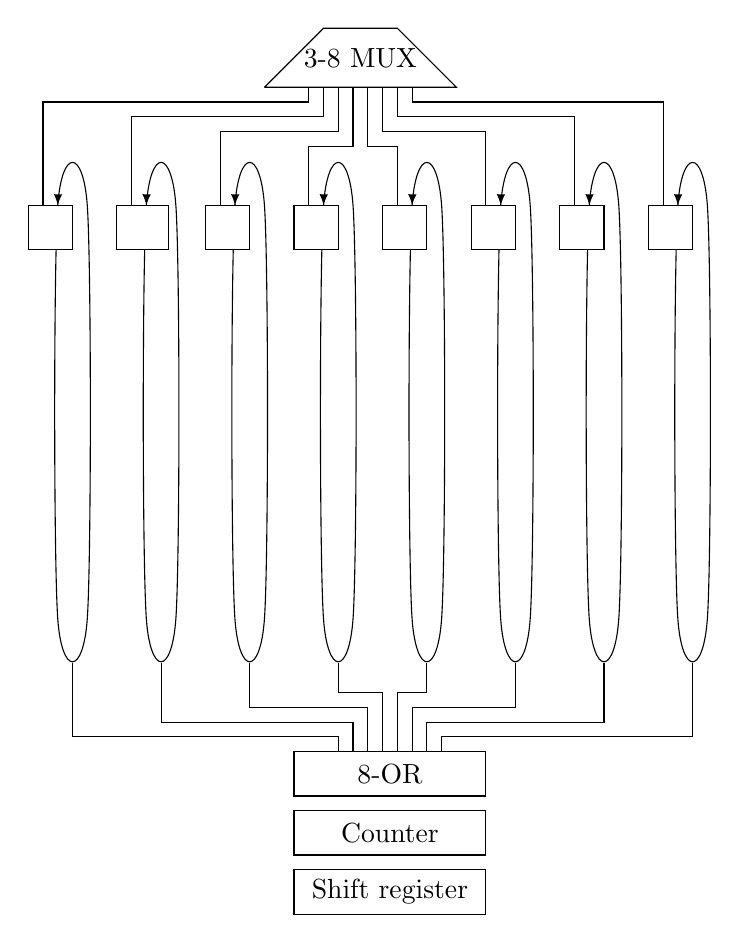
\begin{tikzpicture}[scale=1.5]
%loop
\draw [] plot [smooth cycle] coordinates {(-0.625,-4.5) (-0.625,-1) (-0.375,-1) (-0.375,-4.5)};
\draw [fill=white] (-0.875,-1) rectangle (-0.5,-1.375);
\draw[>=latex,->] (-0.623,-0.9203) -- (-0.625,-1);

%loop
\draw [] plot [smooth cycle] coordinates {(0.125,-4.5) (0.125,-1) (0.375,-1) (0.375,-4.5)};
\draw [fill=white] (-0.125,-1) rectangle (0.3125,-1.375);
\draw[>=latex,->] (0.127,-0.9203) -- (0.125,-1);

%loop
\draw [] plot [smooth cycle] coordinates {(0.875,-4.5) (0.875,-1) (1.125,-1) (1.125,-4.5)};
\draw [fill=white] (0.625,-1) rectangle (1,-1.375);
\draw[>=latex,->] (0.877,-0.9203) -- (0.875,-1);

%loop
\draw [] plot [smooth cycle] coordinates {(1.625,-4.5) (1.625,-1) (1.875,-1) (1.875,-4.5)};
\draw [fill=white] (1.375,-1) rectangle (1.75,-1.375);
\draw[>=latex,->] (1.627,-0.9203) -- (1.625,-1);

%loop
\draw [] plot [smooth cycle] coordinates {(2.375,-4.5) (2.375,-1) (2.625,-1) (2.625,-4.5)};
\draw [fill=white] (2.125,-1) rectangle (2.5,-1.375);
\draw[>=latex,->] (2.377,-0.9203) -- (2.375,-1);

%loop
\draw [] plot [smooth cycle] coordinates {(3.125,-4.5) (3.125,-1) (3.375,-1) (3.375,-4.5)};
\draw [fill=white] (2.875,-1) rectangle (3.25,-1.375);
\draw[>=latex,->] (3.127,-0.9203) -- (3.125,-1);

%loop
\draw [] plot [smooth cycle] coordinates {(3.875,-4.5) (3.875,-1) (4.125,-1) (4.125,-4.5)};
\draw [fill=white] (3.625,-1) rectangle (4,-1.375);
\draw[>=latex,->] (3.877,-0.9203) -- (3.875,-1);

%loop
\draw [] plot [smooth cycle] coordinates {(4.625,-4.5) (4.625,-1) (4.875,-1) (4.875,-4.5)};
\draw [fill=white] (4.375,-1) rectangle (4.75,-1.375);
\draw[>=latex,->] (4.627,-0.9203) -- (4.625,-1);

\draw (1.125,0) -- (1.625,0.5) -- (2.25,0.5) -- (2.75,0) -- (1.125,0) ;

\draw [>=latex, -] (1.875,0) --(1.875,-0.5) -| (1.5,-1);
\draw [>=latex, -] (1.75,0) --(1.75,-0.375) -| (0.75,-1);
\draw [>=latex, -] (1.625,0) --(1.625,-0.25) -| (0,-1);
\draw [>=latex, -] (1.5,0) --(1.5,-0.125) -| (-0.75,-1);

\draw [>=latex, -] (2,0) --(2,-0.5) -| (2.25,-1);
\draw [>=latex, -] (2.125,0) --(2.125,-0.375) -| (3,-1);
\draw [>=latex, -] (2.25,0) --(2.25,-0.25) -| (3.75,-1);
\draw [>=latex, -] (2.375,0) --(2.375,-0.125) -| (4.5,-1);

\node at (1.9375,0.25) {3-8 MUX};
\draw  (1.375,-5.625) rectangle (3,-6)node[pos=.5]{8-OR};
\draw  (1.375,-6.125) rectangle (3,-6.5)node[pos=.5]{Counter};

\draw [>=latex, -] (2.125,-5.625) --(2.125,-5.125) -| (1.75,-4.875);
\draw [>=latex, -] (2,-5.625) --(2,-5.25) -| (1,-4.875);
\draw [>=latex, -] (1.875,-5.625) --(1.875,-5.375) -| (0.25,-4.875);
\draw [>=latex, -] (1.75,-5.625) --(1.75,-5.5) -| (-0.5,-4.875);

\draw [>=latex, -] (2.25,-5.625) --(2.25,-5.125) -| (2.5,-4.875);
\draw [>=latex, -] (2.375,-5.625) --(2.375,-5.25) -| (3.25,-4.875);
\draw [>=latex, -] (2.5,-5.625) --(2.5,-5.375) -| (4,-4.875);
\draw [>=latex, -] (2.625,-5.625) --(2.625,-5.5) -| (4.75,-4.875);

\draw  (1.375,-6.625) rectangle (3,-7)node[pos=.5]{Shift register};
\end{tikzpicture}

\caption{solution with multiple rings and a single counter}
\label{tkz:separateRings}
\end{figure}